\documentclass{article}%
\usepackage{amsmath}
\usepackage{amsfonts}
\usepackage{amssymb}
\usepackage{listings}
\usepackage{graphicx}
\usepackage{tikz}
\usepackage{hyperref}%
\usepackage[a4paper,includeheadfoot,margin=0.5in]{geometry}
\setcounter{MaxMatrixCols}{30}
%TCIDATA{OutputFilter=late$x2$.dll}
%TCIDATA{Version=5.00.0.2552}
%TCIDATA{CSTFile=40 LaTeX article.cst}
%TCIDATA{Created=Thursday, August 21, 2008 14:03:59}
%TCIDATA{LastRevised=Wednesday, October 01, 2014 12:46:33}
%TCIDATA{<META NAME="GraphicsSave" CONTENT="32">}
%TCIDATA{<META NAME="SaveForMode" CONTENT="1">}
%TCIDATA{<META NAME="DocumentShell" CONTENT="Standard LaTeX\Blank - Standard LaTeX Article">}
%TCIDATA{Language=American English}
\newtheorem{theorem}{Theorem}
\newtheorem{acknowledgement}[theorem]{Acknowledgement}
\newtheorem{algorithm}[theorem]{Algorithm}
\newtheorem{axiom}[theorem]{Axiom}
\newtheorem{case}[theorem]{Case}
\newtheorem{claim}[theorem]{Claim}
\newtheorem{conclusion}[theorem]{Conclusion}
\newtheorem{condition}[theorem]{Condition}
\newtheorem{conjecture}[theorem]{Conjecture}
\newtheorem{corollary}[theorem]{Corollary}
\newtheorem{criterion}[theorem]{Criterion}
\newtheorem{definition}[theorem]{Definition}
\newtheorem{example}[theorem]{Example}
\newtheorem{exercise}[theorem]{Exercise}
\newtheorem{lemma}[theorem]{Lemma}
\newtheorem{notation}[theorem]{Notation}
\newtheorem{problem}[theorem]{Problem}
\newtheorem{proposition}[theorem]{Proposition}
\newtheorem{remark}[theorem]{Remark}
\newtheorem{solution}[theorem]{Solution}
\newtheorem{summary}[theorem]{Summary}
\newenvironment{proof}[1][Proof]{\noindent\textbf{#1.} }{\ \rule{0.5em}{0.5em}}

\usepackage{fancyhdr}
\setlength\headheight{26pt}
\pagestyle{fancy}
\lhead{{\footnotesize Final Assignment}}
\rhead{{\footnotesize Christopher Chapline}}
\begin{document}

\section*{Problem 1}
\begin{tabular}{| l | l | l | l |}
    \hline
    $p$ & $\neg p$ & $(\neg p \rightarrow p)$ & $(p \rightarrow (\neg p \rightarrow p))$ \\ \hline
    $T$ & $F$      & $T$                      & $T$ \\ \hline
    $F$ & $T$      & $F$                      & $T$ \\ \hline
\end{tabular}

\section*{Problem 2}

\section*{Problem 3}
\begin{tikzpicture}[scale=0.2]
    \tikzstyle{every node}+=[inner sep=0pt]
    \draw [black] (19.5,-29.8) circle (3);
    \draw (19.5,-29.8) node {$q_0$};
    \draw [black] (31.3,-29.8) circle (3);
    \draw (31.3,-29.8) node {$q_1$};
    \draw [black] (44.5,-29.8) circle (3);
    \draw (44.5,-29.8) node {$q_2$};
    \draw [black] (44.5,-29.8) circle (2.4);
    \draw [black] (22.5,-29.8) -- (28.3,-29.8);
    \fill [black] (28.3,-29.8) -- (27.5,-29.3) -- (27.5,-30.3);
    \draw (25.4,-30.3) node [below] {$a$};
    \draw [black] (29.506,-27.41) arc (244.61966:-43.38034:2.25);
    \draw (29.54,-22.57) node [above] {$b$};
    \fill [black] (32.11,-26.92) -- (32.9,-26.41) -- (32,-25.99);
    \draw [black] (34.3,-29.8) -- (41.5,-29.8);
    \fill [black] (41.5,-29.8) -- (40.7,-29.3) -- (40.7,-30.3);
    \draw (37.9,-30.3) node [below] {$a$};
    \draw [black] (42.855,-27.305) arc (241.12502:-46.87498:2.25);
    \draw (43.4,-22.52) node [above] {$c$};
    \fill [black] (45.48,-26.98) -- (46.3,-26.52) -- (45.43,-26.03);
    \draw [black] (13.4,-29.8) -- (16.5,-29.8);
    \draw (12.9,-29.8) node [left] {$start$};
    \fill [black] (16.5,-29.8) -- (15.7,-29.3) -- (15.7,-30.3);
\end{tikzpicture}

\section*{Problem 4}

\section*{Problem 5}


\end{document}
